\documentclass[12pt,a4paper]{book}
\usepackage[utf8]{inputenc}
\usepackage[T1]{fontenc}
\usepackage{amsmath}
\usepackage{amsfonts}
\usepackage{amssymb}
\usepackage{graphicx}
\usepackage{float}
\usepackage{listings}
\usepackage{color}
\usepackage{lscape}
\usepackage{hyperref}

\definecolor{dkgreen}{rgb}{0,0.6,0}
\definecolor{gray}{rgb}{0.5,0.5,0.5}
\definecolor{mauve}{rgb}{0.58,0,0.82}

\lstset{frame=tb,
	language=Java,
	aboveskip=3mm,
	belowskip=3mm,
	showstringspaces=false,
	columns=flexible,
	basicstyle={\small\ttfamily},
	numbers=none,
	numberstyle=\tiny\color{gray},
	keywordstyle=\color{blue},
	commentstyle=\color{dkgreen},
	stringstyle=\color{mauve},
	breaklines=true,
	breakatwhitespace=true,
	tabsize=3
}

\begin{document}
\title{\textbf{AQA 2020-2021 Project: Fluid Dynamics Simulator}}
\author{Anastasios Zeniou}

\date{}
\maketitle
\tableofcontents

\pagebreak


\chapter{Analysis}
\section{Preamble}
In the following documentation, I will explain the conception, creation and improvement of my Fluid Dynamics simulation. This project is heavily based on a paper by Jos Stam published in 2003 named "Real-Time Fluid Dynamics for Games" and this project would not be fruitful without it. I cannot claim that my project is an original idea and entirely self-thought, but only a derivative of said paper. My focus was implementing the mathematical solver proposed by the paper in a visual environment. To do this I used processing.js, which is a tool of simplification for creating visuals using Java. This decision was intentional, as I found that had I made my project in python, C++ and Java, it would've been unnecessarily difficult. The paper itself has code snippets in C and so a translation was required. Like in the preamble of the paper, it is to be made clear that the solver is not focused on accuracy, but speed and reliability by finding approximate solutions to the famous Navier-Stokes Equations:

\begin{equation*}\label{nseq:vel}
	\dfrac{\partial u}{\partial t} = -(u\cdot \nabla)u + v{\nabla}^2u + f
\end{equation*}
\begin{equation*}\label{nseq:den}
	\dfrac{\partial \rho}{\partial t} = -(u \cdot \nabla)\rho + k{\nabla}^2\rho + S
\end{equation*}

\section{Research}
According to my preliminary understanding of the Navier-Stokes equations, they represent a mathematical formulation of the velocity vector field and density field. That means that they can predict the velocity and density (of a number) of gases at all infinitesimally small places in space after infinitesimally small advances in time. They are notoriously difficult to solve and in fact, whoever does solve them will win 1 million dollars. For the purpose of this documentation, the top and bottom equation both have 3 terms that velocity and density of particles at any given point depend on. This similarity, as stated in the paper "was instrumental in the development of our algorithms". The reader and I are not expected to understand these equations fully. However, it must be made clear that we are not considering one fluid, but two. One we can think of the first as the background and what we are solving is the density of the second fluid. A simile I like for this is that we are considering the amount of dye spread around in some other fluid like water.


\section{In-depth explanation of the solver}
To start, the solver is based on computational grids, which means that we conceptually use 2D/3D arrays to approximate a velocity vector field and density through it. For the sake of efficiency/time complexity, we create 1D arrays with size (N+2)*(N+2) instead of 2D arrays, where the +2 accounts for boundary conditions. Using a macro from C translated to a function in Java, we can easily and quickly access all elements of the array. Similarly to ADC, the cells represent a sample of the density of the fluid at a square physical space of length 1/N every time advance \verb|dt| of the visually displayed snapshots.\\
\\
The bottom equation formulates the density at each cell in the 1D density array. The three terms mean the density will follow the velocity field, the density will diffuse at a certain rate and the density may increase due to external sources in that order correspondingly. The solver will work in a way such that the next snapshot will add these three terms on each cell of the current snapshot. External sources in this case mean the mouse. The user can left click to add fluid in the specific fluid configuration or right click to remove fluid. Diffusion is done by exchanging density values with its neighbouring cells, namely the top, bottom, left and right cell. Therefore its density decreases because it is spread to the grid cells and increases its density also due to its grid cells exchanging density. The net result will be negative in the original cell and positive in the grid cells, mimicking diffusion. A literal implementation of this is however faulty and hence we use an alternative method of determining the value of the cell following diffusion using \textbf{Matrix Inversion}. As stated in the paper, the standard matrix inversion routine is unnecessary because the majority of elements are zero in said matrix. Alternatively we implement the Gauss-Seidel relaxation, which is an iterative method of finding the inverse of a matrix and that in turn makes the diffusion function stable. Finally the remaining term relating the velocity vector field to the density (called \emph{advection}) is implemented using linear interpolation based on the premise that at the centre of each cell there exists a particle.\\
\\
The similarity of the equations allows us to use the same functions used for the density solver, for the velocity vector field solver. The corresponding three terms in the top equation are the addition of forces, viscous diffusion and self-advection. A highlighted part of the solver is a function used to force the velocity to be mass conserving (\verb|Project()|), which is an important property of real life fluids that must be taken into consideration, otherwise the solver would be unstable and unrealistic. The reader will notice that the function \verb|SetBnd()| recurs frequently in the code. This aptly named function is used to take care of boundary conditions, essentially making sure that cells can't exchange values with the boundary cells in the grid. The literal purpose of this is to think the grid as a box from which no fluid can exit. A limitation of this solver, not that of processing power, but of accuracy is observable because simulated fluids dampen unrealistically quickly.

\section{Object Oriented Programming Planning}
In order to utilize the solver in the conventionally correct way, I create two files; the main file that oversees the simulation of the fluid, listens for key strokes etc, and the Fluid file, which contains some global variables and the Fluid class. The class Fluid contains the mathematical simulation of the fluid along with its rendering.



\chapter{Code}

\section{Code explanation}

Firstly, I will go over \verb|Fluid.pde|, which is where the solver is found. 
\begin{lstlisting}
	final int N=64;
	final int GRIDSIZE = (N+2)*(N+2);
	final int SCALE = 15;
	
	float dt = 0.04;
	final float max_dt = 0.1;
	final float min_dt = 0.002;
	
	int IX(int i, int j){
		return i + (N+2)*j; 
	}
\end{lstlisting}
Here I declare important global variables such as \verb|N| and \verb|dt| which mean the length of the size of the grid and the time step correspondingly. \verb|max_dt| and \verb|min_dt| exist due to my added functionality, allowing the user to alter the time step \verb|dt| between \verb|dt_min| and \verb|dt_max|, which is allowed because the solver is a stable one and will not "blow up" with extreme values for \verb|dt|. \verb|N| represents the length of the square grid in pixels, hence there will be $ 64*64= 4096$ (stored in \verb|GRIDSIZE|) pixels displayed. Instead of simulating more pixels to get a bigger simulation window, I instead use scale \verb|SCALE| meant to increase the "size" of the pixels shown on screen, mimicking a greater number of pixels. This comes with the advantage of requiring a lot less processing power, while still being a big window. We can also see the translated macro function IX.\\
\\
\begin{lstlisting}
	class Fluid{
		
		float dt;
		float diff;
		float visc;
		int size;
		
		float[] u;
		float[] v;
		float[] u_prev;
		float[] v_prev;
		
		float[] dens;
		float[] dens_prev;
		
		Fluid(float diffusion, float viscosity, float dtime){
			this.diff = diffusion;
			this.visc = viscosity;
			this.dt = dtime;
			
			this.dens_prev = new float[GRIDSIZE];
			this.dens = new float[GRIDSIZE];
			
			this.u = new float[GRIDSIZE];
			this.u_prev = new float[GRIDSIZE];
			this.v = new float[GRIDSIZE];
			this.v_prev = new float[GRIDSIZE];
		}
\end{lstlisting}
This code simply initializes the velocity and density fields grids. \verb|u| and \verb|v| is the x-component and y-component of the velocity for each cell. The technique explained in the preamble, namely the iterative method of Matrix Inversion, requires a previous snapshot of the velocity field, for which \verb|u_prev| and \verb|v_prev| are responsible; same goes for density. All the fluids are made to be objects of the class \verb|Fluid| and as we will see later, modifying the value of \verb|dt| inherently changes the fluid simulated and clears the canvas. I tried to find a workaround in this but I believe it is impossible to as it is inherent to the solver.
\begin{lstlisting}
	  void step(float dtime){
		VelStep(u,v,u_prev,v_prev,visc,dtime);
		DensStep(dens,dens_prev,u_prev,v_prev,diff);
	}
	
	void SetBnd(int b, float[] x){
		
		for (int i=1 ; i<=N ; i++ ) {
			x[IX(0 ,i)] = (b==1) ? -x[IX(1,i)] : x[IX(1,i)];
			x[IX(N+1,i)] = (b==1) ? -x[IX(N,i)] : x[IX(N,i)];
			x[IX(i,0 )] = (b==2) ? -x[IX(i,1)] : x[IX(i,1)];
			x[IX(i,N+1)] = (b==2) ? -x[IX(i,N)] : x[IX(i,N)];
		}
		x[IX(0 ,0 )] = 0.5*(x[IX(1,0 )]+x[IX(0 ,1)]);
		x[IX(0 ,N+1)] = 0.5*(x[IX(1,N+1)]+x[IX(0 ,N )]);
		x[IX(N+1,0 )] = 0.5*(x[IX(N,0 )]+x[IX(N+1,1)]);
		x[IX(N+1,N+1)] = 0.5*(x[IX(N,N+1)]+x[IX(N+1,N )]);
	}
\end{lstlisting} 
\verb|SetBnd| is responsible for taking care of the boundary conditions, namely "mirroring" the value of \verb|float[] x| at the boundary conditions. This array is named x because it can be made to take the value of both the velocity and the density fields from the rest of the code. This is what the paper was referring to when it said that the solver takes advantage of the similarities between the two equations. \verb|step| simply calls the solver every time step |dt| and calls the functions \verb|DensStep()| and \verb|VelStep()|:
\begin{lstlisting}
	  void DensStep (float[] x, float[] x0, float[] u, float[] v, float diff ){
		Diffuse ( 0, x0, x, diff);
		Advect ( 0, x, x0, u, v);
	}
	
	void VelStep(float[] u, float[] v, float[] u0, float[] v0, float visc, float dt){
		float[] tmp;
		
		
		tmp = u0; u0 = u; u=tmp;
		Diffuse(1,u,u0,visc);
		
		tmp = v0; v0 = v; v=tmp;
		Diffuse(2,v,v0,visc);
		
		Project(u,v,u0,v0);
		tmp = u0; u0 = u; u=tmp;
		tmp = v0; v0 = v; v=tmp;
		
		Advect(1,u,u0,u0,v0); Advect(2,v,v0,u0,v0);
		
		Project(u,v,u0,v0);
		
	}

\end{lstlisting}

\begin{lstlisting}
	  void AddDensity(int x, int y, float amount){
		int index = IX(x,y);
		this.dens[index] += amount;
	}
	
	void AddVelocity(int x, int y, float amountX, float amountY){
		int index = IX(x,y);
		this.v[index] += amountX;
		this.u[index] += amountY;
	}
	
\end{lstlisting}
These functions add (and subtract) to the density and velocity fields and they are called from the other file, where the mouse is tracked and the "forces" are added. This concludes the first term on both of the Navier-Stokes equations.
\begin{lstlisting}
	  void Diffuse(int b, float[] x, float[] x0, float diff){
		
		float a = dt*diff*N*N;
		
		for(int k=0;k<20;k++){
			for(int i=1;i<=N;i++){
				for(int j=1;j<=N;j++){
					x[IX(i,j)] = (x0[IX(i,j)] + a*(x[IX(i-1,j)] + x[IX(i+1,j)] + x[IX(i,j-1)] + x[IX(i,j+1)]))/(1+4*a);
				}
			}
			SetBnd(b,x);
		}
		
	}
\end{lstlisting}
This function takes care of density diffusion. Similarly to the previous function, this function (or because it is a void function, a subroutine) takes parameters \verb|float[] x| and \verb|float[] x0| represent two different snapshots of the density/velocity field. The technique of finding the new values of density/velocity mentioned in the preamble is implemented, while taking care of boundary conditions. This concludes the second term of both equations, namely diffusion and viscous diffusion.
\begin{lstlisting}
	  void Advect(int b, float[] d, float[] d0, float[] u, float[] v){
		
		int i, j, i0, j0, i1, j1;
		float x, y, s0, t0, s1, t1, dt0;
		
		dt0 = dt*N;
		
		for(i=1;i<=N;i++){
			for(j=1;j<=N;j++){
				x = i-dt0*u[IX(i,j)]; y = j-dt0*v[IX(i,j)];
				if (x<0.5) x=0.5; if (x>N+0.5) x=N+ 0.5; i0=int(x); i1=i0+1;
				if (y<0.5) y=0.5; if (y>N+0.5) y=N+ 0.5; j0=int(y); j1=j0+1;
				s1 = x-i0; s0 = 1-s1; t1 = y-j0; t0 = 1-t1;
				d[IX(i,j)] = s0*(t0*d0[IX(i0,j0)]+t1*d0[IX(i0,j1)])+ s1*(t0*d0[IX(i1,j0)]+t1*d0[IX(i1,j1)]);
				
				
			}
		}
		SetBnd(b,d);
		
	}
\end{lstlisting}
The third and final term on both the equations, meaning the advection and self-advection is handled by this subroutine, which I still cannot wrap my head around (Then again, I am not supposed/expected to). The function to force the velocity field to be mass conserving (\verb|Project()|) is:
\begin{lstlisting}
	  void Project(float[] u, float[] v, float[] p, float[] div){
		
		int i,j,k;
		float h;
		
		h = 1.0/N;
		for(i=1;i<=N;i++){
			for(j=1;j<=N;j++){
				div[IX(i,j)] = -0.5*h*(u[IX(i+1,j)]-u[IX(i-1,j)]+ v[IX(i,j+1)]-v[IX(i,j-1)]);
				p[IX(i,j)] = 0;
			}
		}
		SetBnd(0,div); SetBnd(0,p);
		
		for ( k=0 ; k<20 ; k++ ) {
			for ( i=1 ; i<=N ; i++ ) {
				for ( j=1 ; j<=N ; j++ ) {
					p[IX(i,j)] = (div[IX(i,j)]+p[IX(i-1,j)]+p[IX(i+1,j)]+ p[IX(i,j-1)]+p[IX(i,j+1)])/4;
				}
			}
			SetBnd(0, p);
		}
		
		for ( i=1 ; i<=N ; i++ ) {
			for ( j=1 ; j<=N ; j++ ) {
				u[IX(i,j)] -= 0.5*(p[IX(i+1,j)]-p[IX(i-1,j)])/h;
				v[IX(i,j)] -= 0.5*(p[IX(i,j+1)]-p[IX(i,j-1)])/h;
			}
		}
		SetBnd(1, u); SetBnd(2, v);
		
	}
\end{lstlisting}

Having finished with the solver, only the rendering remains. The subroutine \verb|RenderD()| that isn't included in the paper is responsible for the rendering of the density field, which is the field visible to us, much like how we see the colour of the smoke, which is dependent on its concentration, rather than the velocities of the smoke particles.
\begin{lstlisting}
	void RenderD(boolean dark, boolean code){
		noStroke();
		colorMode(HSB,100);
		
		for(int i=0;i<N;i++){
			for(int j=0;j<N;j++){
				int x = i * SCALE;
				int y = j * SCALE;
				
				float dr = this.dens[IX(i,j)];
				if(dark == true && code == true){fill(dr,255,dr);}
				else if (dark == false && code == false){fill(255,dr,255);}
				else if (dark == true && code == false){fill(0,dr,dr);}
				else if (dark == false && code == true){fill(dr,dr,255);}
				
				square(x,y,SCALE);
			}
		}
		
		
	}
\end{lstlisting}
Boolean dark and code each mean store the choice of the user for the background to be dark or light and for the density of the cells to be colour-coded or not, respectively. Each cell is represented by a square with scale \verb|GRIDSIZE|. \\
\\
Moving onto the "master file" \verb|sketch_201122a.pde|:
\begin{lstlisting}
	import static javax.swing.JOptionPane.*;
	
	Fluid fluid;
	JSONArray fluids;
	
	int choice = 0;
	String FluidName;
	Float FluidDiffusion, FluidViscosity;
	int brush_size = 1000;
	final int FrameRateCap=120;
	
	final int max_brush_size = 4000;
	final int min_brush_size = 100;
	boolean dark = true;
	boolean colorcode = true;
	
	int DSCALE = 100;
	
	
\end{lstlisting}
I import a library for the display of a message showing the key bindings for the functionalities of the program, as I found it virtually impossible to remember all of them. I create an instance of the \verb|Fluid| file and create global variables \verb|choice,FluidName,FluidDiffusion,FluidViscosity| to take the values from the JSON file containing the fluid configurations. Because I observed that the differences between fluid configurations were minute thus rendering my efforts to add realism to the program null, I create variable \verb|DSCALE| used to augment the viscosities and diffusion values and thus augment the differences between the values of the different fluid configurations. \verb|brush_size| and the minimum and maximum handle the amount of density the user can add/subtract and can be changed with the mouse wheel, which we will later see. \verb|FrameRateCap| is the maximum FPS the program will run at, \verb|choice| is the default fluid configuration choice that also stores the user choice and the rest are self-explanatory.\\
\\
Then follows the \verb|settings()| function per the syntax of processing.js:
\begin{lstlisting}
	void settings(){
		size(N*SCALE,N*SCALE);
	}
\end{lstlisting}
and \verb|setup()|:
\begin{lstlisting}
	void setup(){
		frameRate(FrameRateCap);
		InitUI();
		
		fluids = loadJSONArray("data/fluids.json");
		GetFluid(choice);
	}
	
	
\end{lstlisting}
where I enforce the frame rate cap, load the UI message at the start and the JSON file, and choose the fluid configuration to be displayed, the default value being 0 (\verb|int choice=0|). \\
\\

The UI message at the start, shows the different key binds and explains the information to be shown on the simulation screen, using the imported library at the start of the code
\begin{lstlisting}
	void InitUI(){  
		String message = "The key bindings for the simulation are as follows:\nd : Toggle Dark Mode";
		message += "\nc : Toggle Color Coding\nn : Clear\nf : Cycle Through Fluids";
		message += "\nDrag Left Click : Add Fluid\nDrag Right Click : Remove Fluid\nScroll : Change Brush Size";
		message += "\ns : Lower Simulation Speed\na : Increase Simulation Speed";
		message += "\n\nThe legend of the UI is:\nFPS (" + str(FrameRateCap) + " max)  /  Brush Size /  Speed of Simulation  /  Fluid Configuration";
		
		showMessageDialog(null, message, "UI Help", INFORMATION_MESSAGE);
		
		
	}
\end{lstlisting}
\verb|RenderUI()| takes care of the rendering of the information shown on the screen, such as the FPS, the brush size, the time step \verb|dt| and the fluid configuration.\\
\\
The following function handles erroneous values for the position of \verb|mouseX| and \verb|mouseY| - the x and y position of the pointer relative to the upper left hand corner of the window - when the pointer is outside the window.
\begin{lstlisting}
	int ConstrainMouse(int maxV, int val){
		if(val >= maxV){
			return maxV - 1;
		}
		if(val<=0){
			return 1; 
		}
		return val;
	}
\end{lstlisting}
\verb|GetFluid()| simply manages the \verb|Fluid.pde| file by reading the JSON file at the given \verb|choice| and creating a new instance of the file called \verb|fluid|, which is where the viscosity and diffusion are augmented according to \verb|DSCALE|.

\begin{lstlisting}
	void GetFluid(int newchoice){
		choice = newchoice%fluids.size();
		JSONObject fluids_choice = fluids.getJSONObject(choice);
		
		FluidName = fluids_choice.getString("configuration");
		FluidDiffusion = fluids_choice.getFloat("diffusion");
		FluidViscosity = fluids_choice.getFloat("viscosity");
		
		fluid = new Fluid(FluidDiffusion*DSCALE, FluidViscosity*DSCALE, dt);
	}
	
\end{lstlisting}

\verb|SetSimulationSpeed()| is the function that handles the change in \verb|dt| and calls \verb|GetFluid()|.
\begin{lstlisting}
	void SetSimulationSpeed(boolean increase){
		if(increase){
			dt+=0.002;
			if(dt>max_dt){dt=max_dt;}
		}
		else{
			dt-=0.002;
			if(dt<min_dt){dt=min_dt;}
		}
		GetFluid(choice);
	}
\end{lstlisting}
To check if the user pressed left or right click, a function is needed. I use the built-in function \verb|mouseDragged| for reasons outlined in the System Testing chapter. This subroutine is called every time the mouse is dragged. Additionally, I am able to utilize \verb|mouseX,pmouseX| and the corresponding for Y to determine the direction in which the pointer is dragged, allowing me to trace it in the velocity vector field or velocity of the "background" fluid. 
\begin{lstlisting}
	void mouseDragged(){
		
		float amountX = mouseX - pmouseX;
		float amountY = mouseY - pmouseY;
		
		int maxX = int(width/SCALE) - 1;
		int maxY = int(height/SCALE) - 1;
		
		if (mousePressed && (mouseButton == LEFT)){
			fluid.AddDensity(ConstrainMouse(maxX,mouseX/SCALE) , ConstrainMouse(maxY, mouseY/SCALE) , brush_size);
			fluid.AddVelocity(ConstrainMouse(maxX,mouseX/SCALE) , ConstrainMouse(maxY, mouseY/SCALE) , amountX*10, amountY*10);
		}
		if(mousePressed && (mouseButton == RIGHT)){
			fluid.AddDensity(ConstrainMouse(maxX,mouseX/SCALE) , ConstrainMouse(maxY, mouseY/SCALE), -brush_size);
		}
		
	}
	
\end{lstlisting}
which is where I call \verb|AddDensity()| and \verb|AddVelocity()| and can "suck out" the fluid with right click. I check if the left/right click is being pressed and add density and velocity for a left click and remove density - or rather add the negative value of \verb|brush_size| to the density field.
\begin{lstlisting}
	void keyPressed(){
		if(key=='d'){dark = !dark;}
		if(key=='c'){colorcode = !colorcode;}
		if(key=='n'){GetFluid(choice);}
		if(key=='f'){GetFluid(choice+1);}
		if(key=='a'){SetSimulationSpeed(true);}
		if(key=='s'){SetSimulationSpeed(false);}
	}
	
	void mouseWheel(MouseEvent event){
		float e = -1*event.getCount();
		brush_size += e*20;
		if(brush_size <= min_brush_size){brush_size=min_brush_size;}
		if(brush_size>=max_brush_size){brush_size=max_brush_size;}
	}
	
\end{lstlisting}
Both of the above functions take care of the key bindings and change the brush size according to movement from the mouse wheel. Both of them are built-in functions, however, and are only triggered when a key is pressed and the mouse wheel is moved, correspondingly.\\
\\
Finally, per the syntax of processing.js, the \verb|draw()| function is called, where the is canvas is reset and the next snapshot is displayed by calling the function \verb|RenderD()| from the file \verb|Fluid.pde| and the UI is displayed
\begin{lstlisting}
	void draw(){
		background(0);
		
		fluid.step(dt);
		fluid.RenderD(dark,colorcode);
		
		RenderUI();
		
	}
\end{lstlisting}


\section{Hierarchy Diagram}
It is my hope that the following Diagram simplifies the perplexity of the program. The arrows are only for unambiguity in the connection of methods.
\begin{landscape}
\begin{figure}[H]
	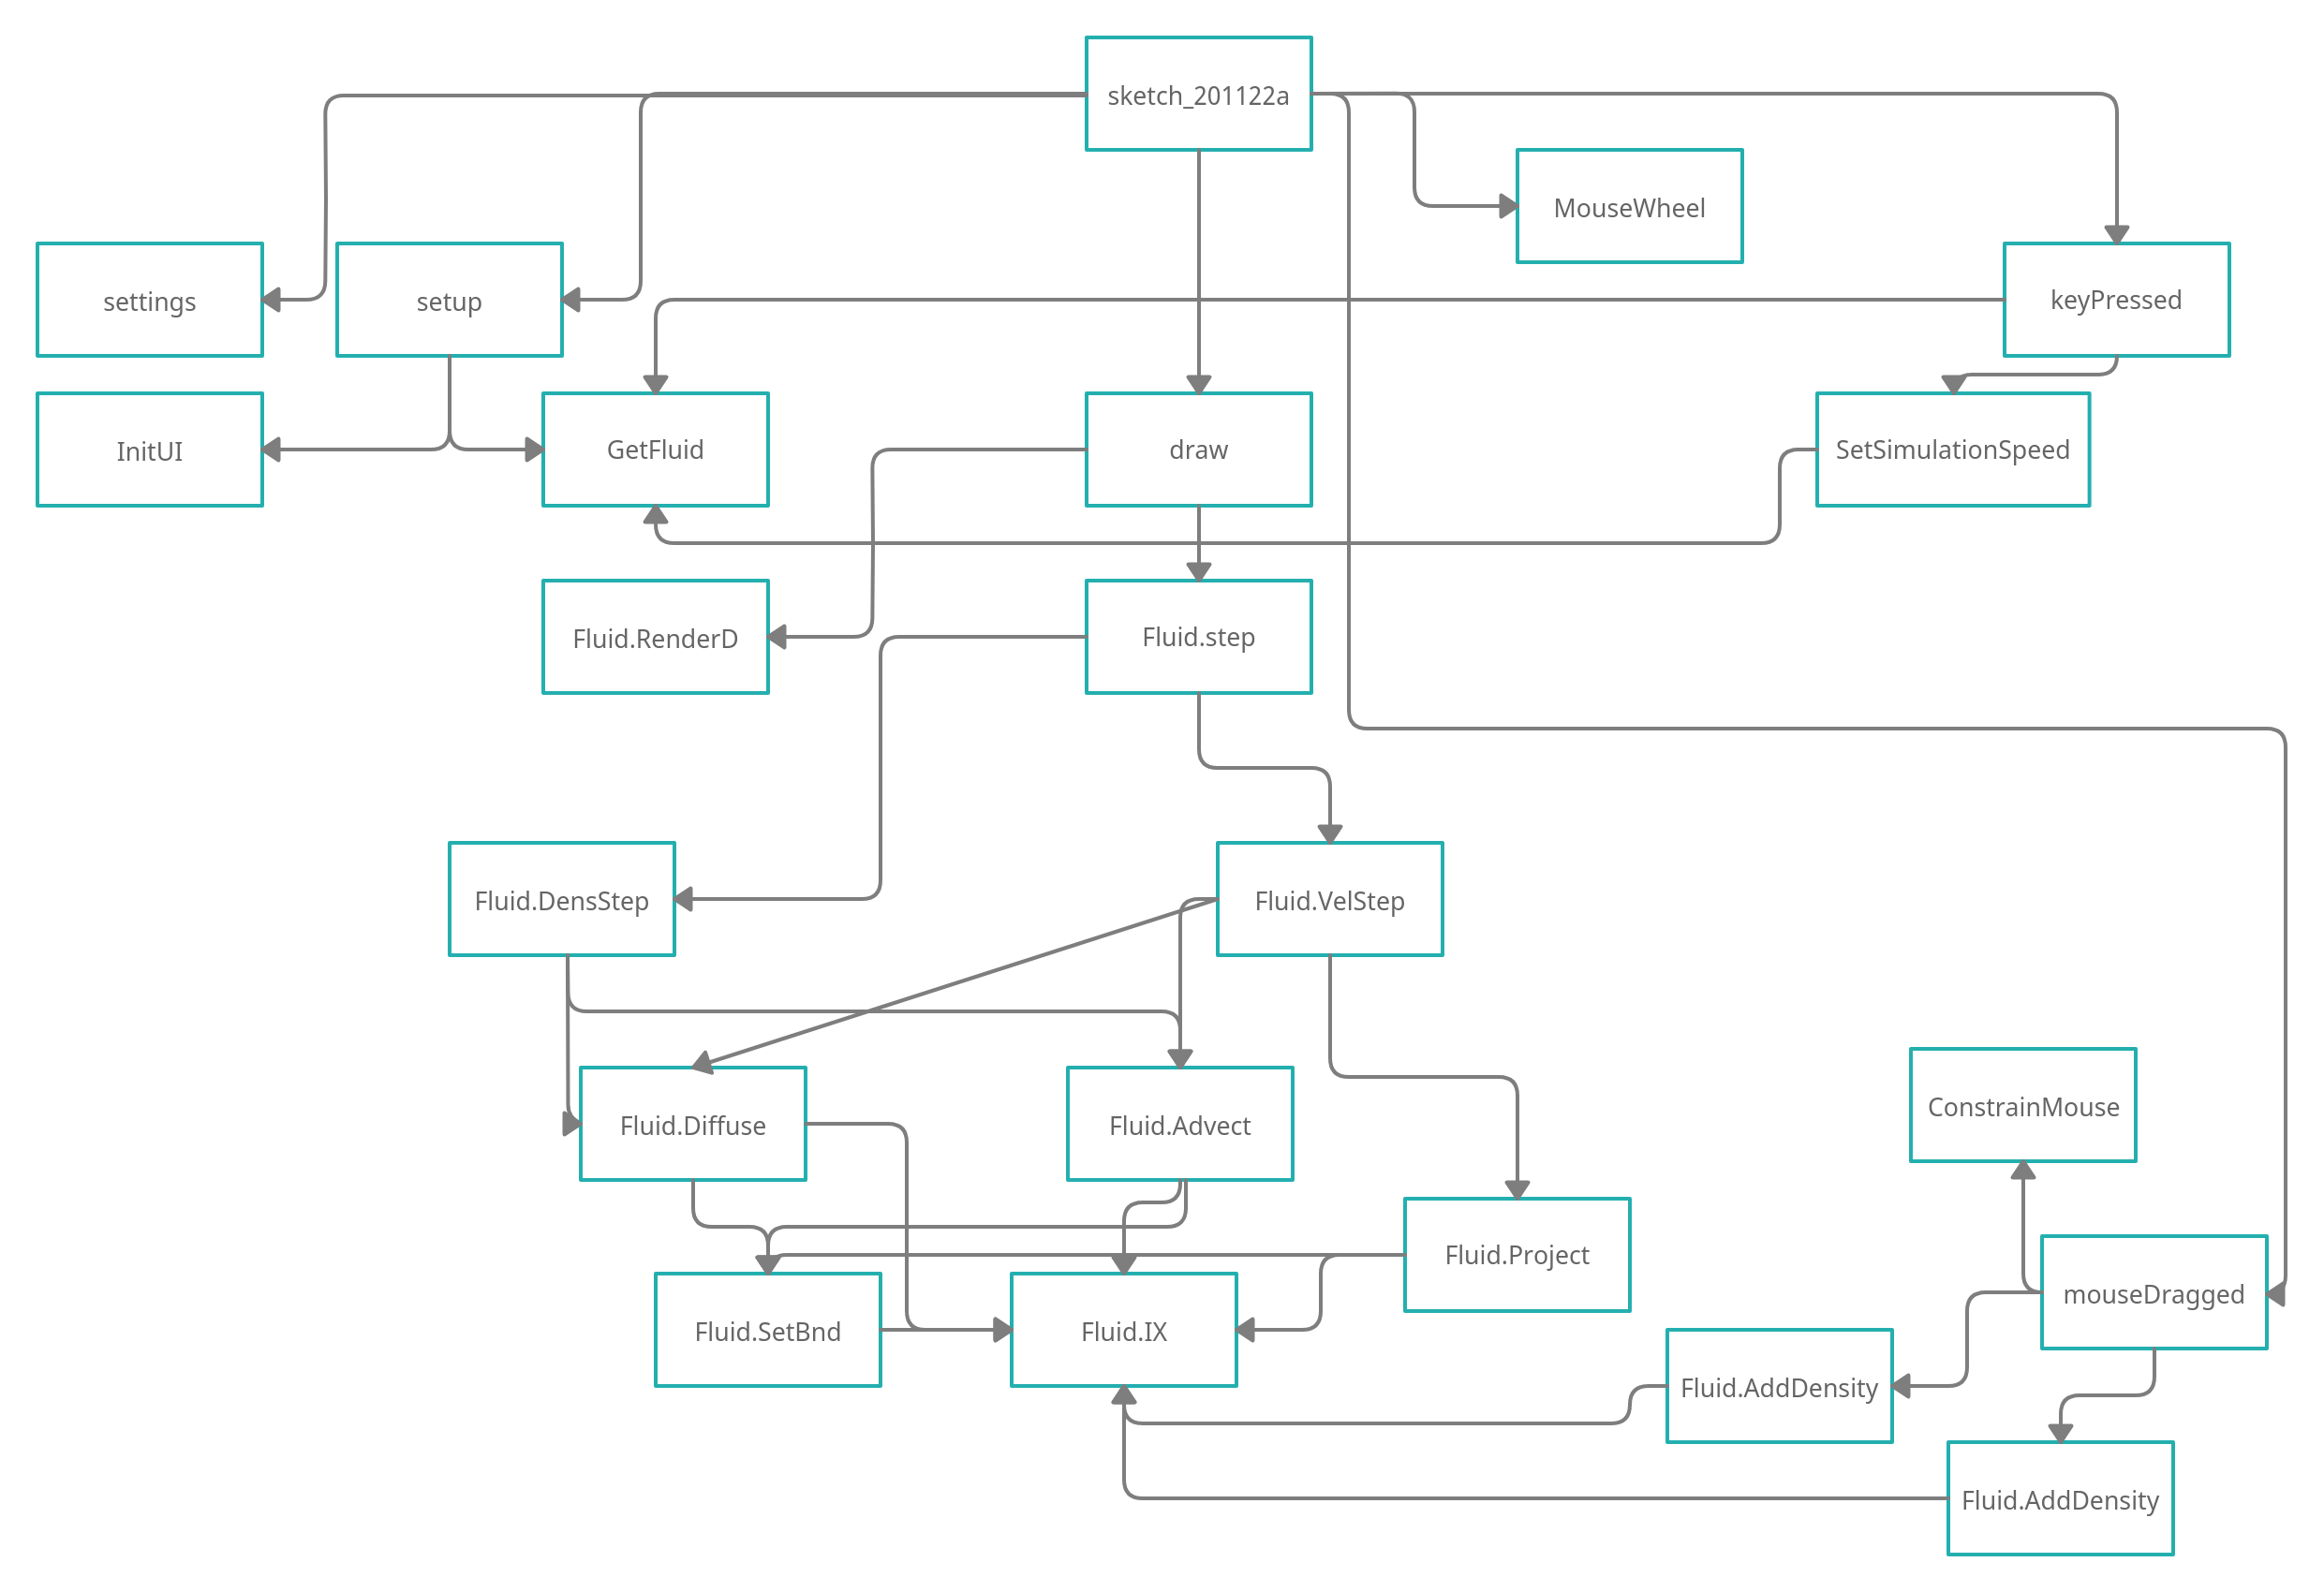
\includegraphics[scale=0.2]{pics/Hierarchy.png}
\end{figure}
\end{landscape}


\chapter{Operation Example}
At the start of the program (.exe for Windows, executable for Linux), the user is met with the panel explaining the key bindings and the information of the UI:

\begin{figure}[H]
	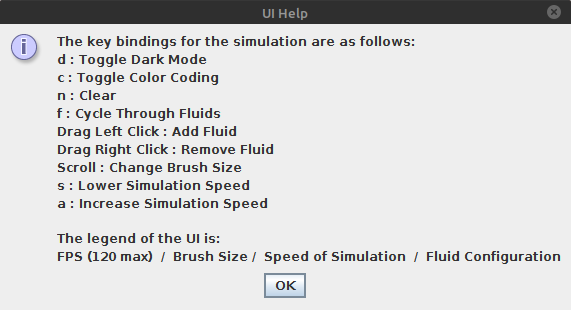
\includegraphics[scale=0.5]{pics/0.png}
\end{figure}

\pagebreak

Please note the FPS is never this low. The user is then met with an empty black screen on the default fluid configuration. As it can be seen in the Code Snippets, there are 6 fluid configurations.

\begin{figure}[H]
	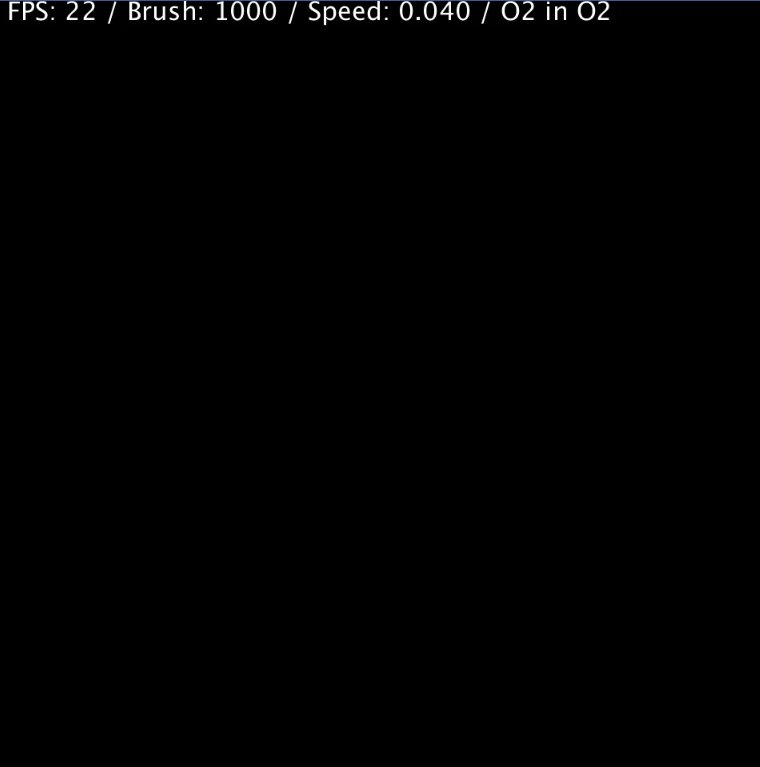
\includegraphics[scale=0.5]{pics/blank.png}
\end{figure}

\pagebreak
The user then left clicks and drags to add density with the default brush size 1000, dt=0.04 and O2 in O2.

\begin{figure}[H]
	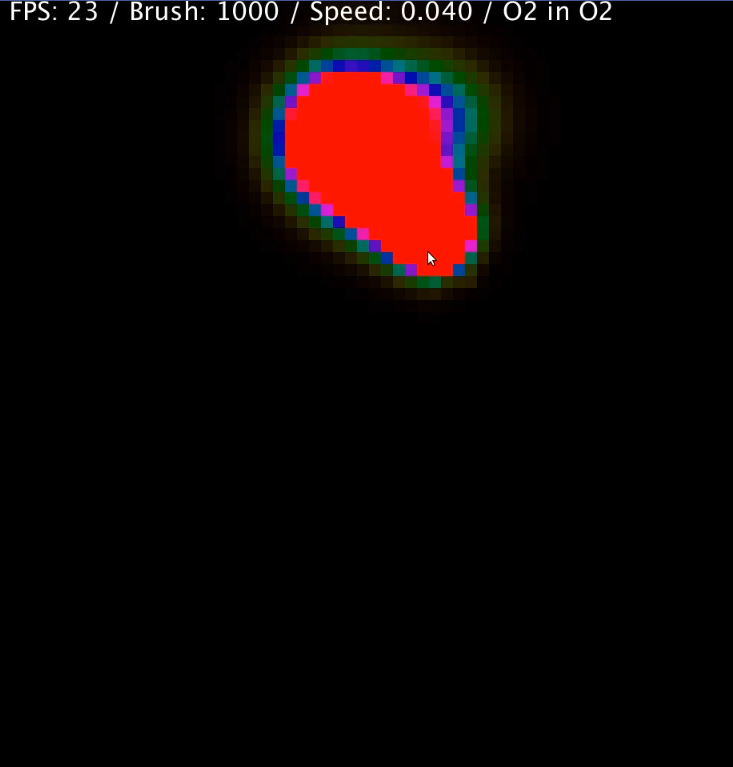
\includegraphics[scale=0.5]{pics/1.png}
\end{figure}

\pagebreak
The fluid then spreads and follows the velocity vector field.

\begin{figure}[H]
	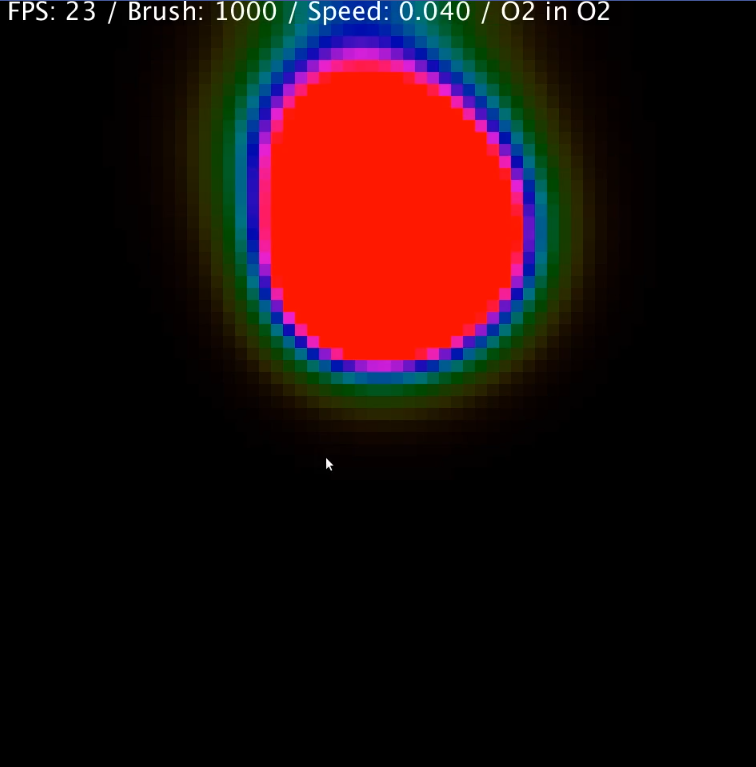
\includegraphics[scale=0.5]{pics/2.png}
\end{figure}

\pagebreak
The user, of course, can add density in multiple places.

\begin{figure}[H]
	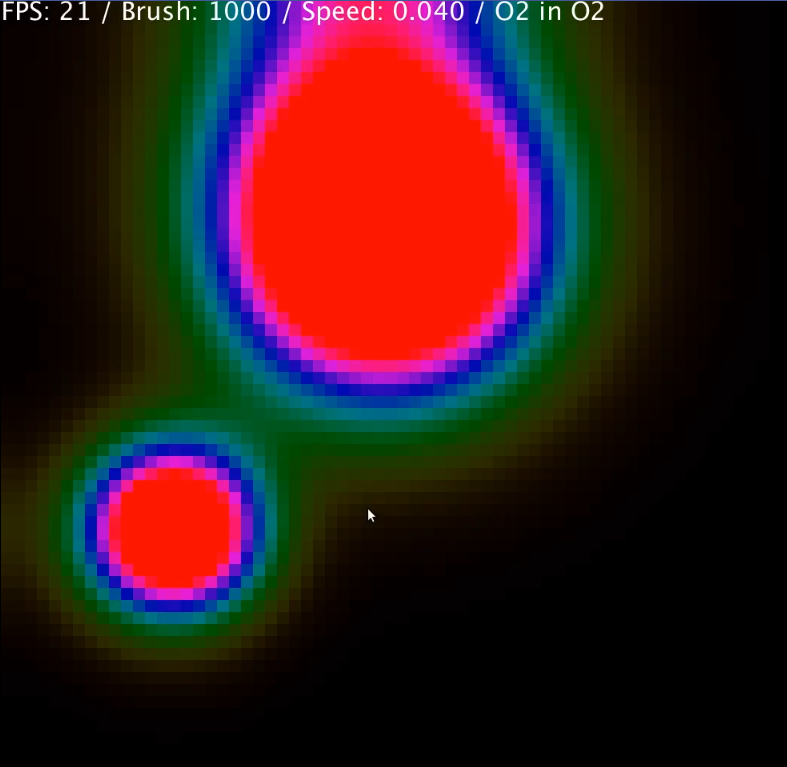
\includegraphics[scale=0.5]{pics/3.png}
\end{figure}

\pagebreak
And remove density by right clicking and dragging.

\begin{figure}[H]
	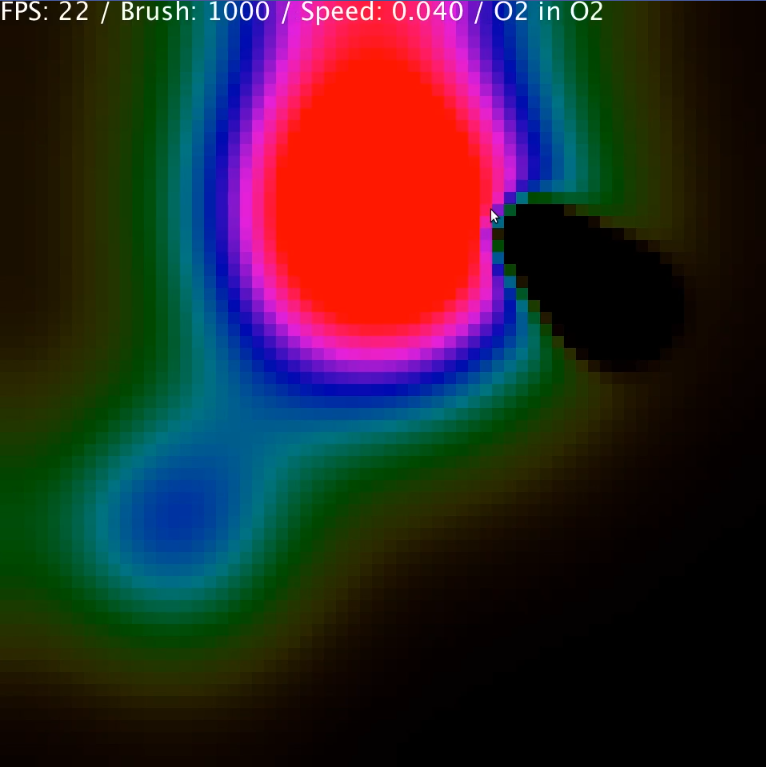
\includegraphics[scale=0.5]{pics/4.png}
\end{figure}

\pagebreak
This won't add to the velocity vector field, and the lack of density will "consume" the other density.

\begin{figure}[H]
	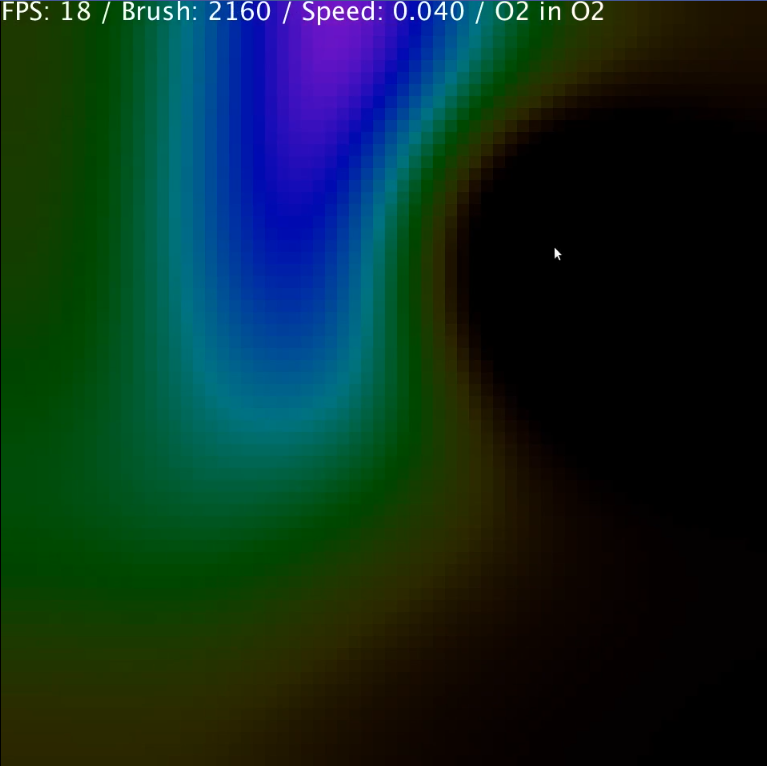
\includegraphics[scale=0.5]{pics/5.png}
\end{figure}

\pagebreak
Spinning the wheel upwards increases the brush size up to 4000 with increments of 100.

\begin{figure}[H]
	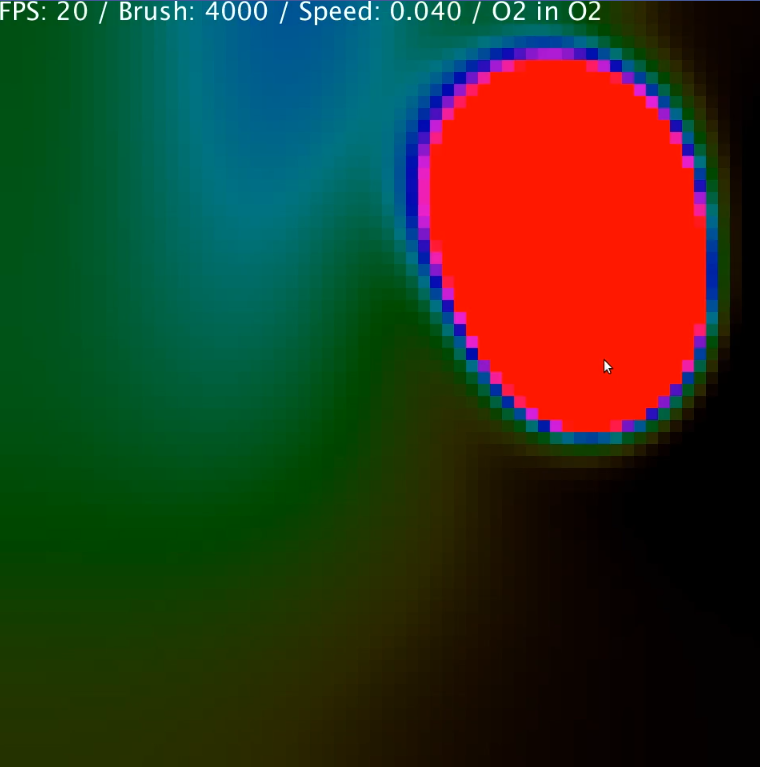
\includegraphics[scale=0.5]{pics/6.png}
\end{figure}


\pagebreak
This max brush size will add a lot of density that will go up to the boundary cells (screenshotting a bit to the right to see that the density is blocked by the boundary cells).

\begin{figure}[H]
	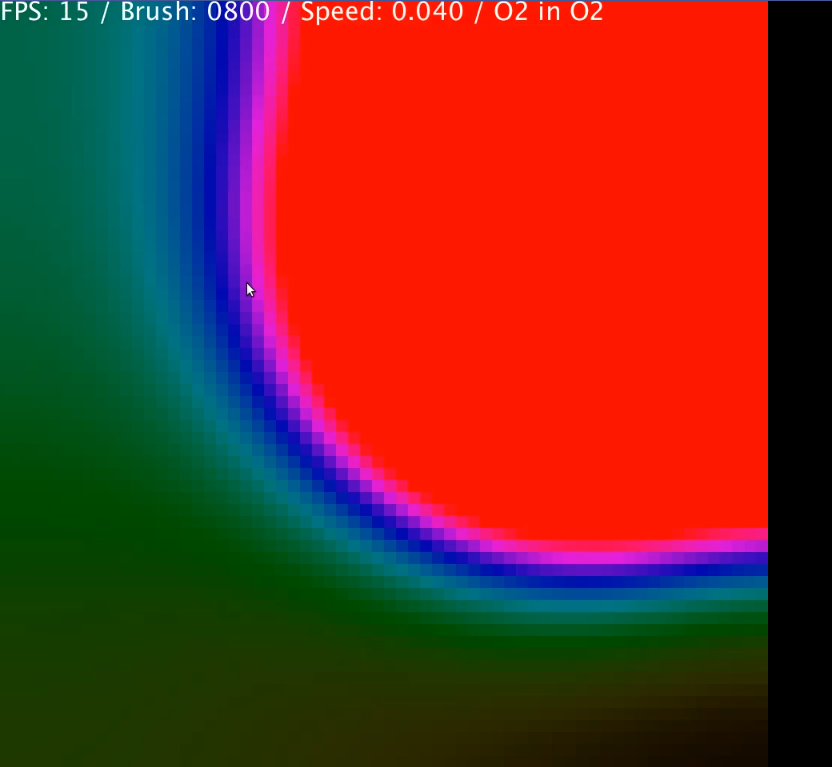
\includegraphics[scale=0.5]{pics/7.png}
\end{figure}

\pagebreak
Spinning the wheel down down to brush size 100 makes the amount of density added very small.

\begin{figure}[H]
	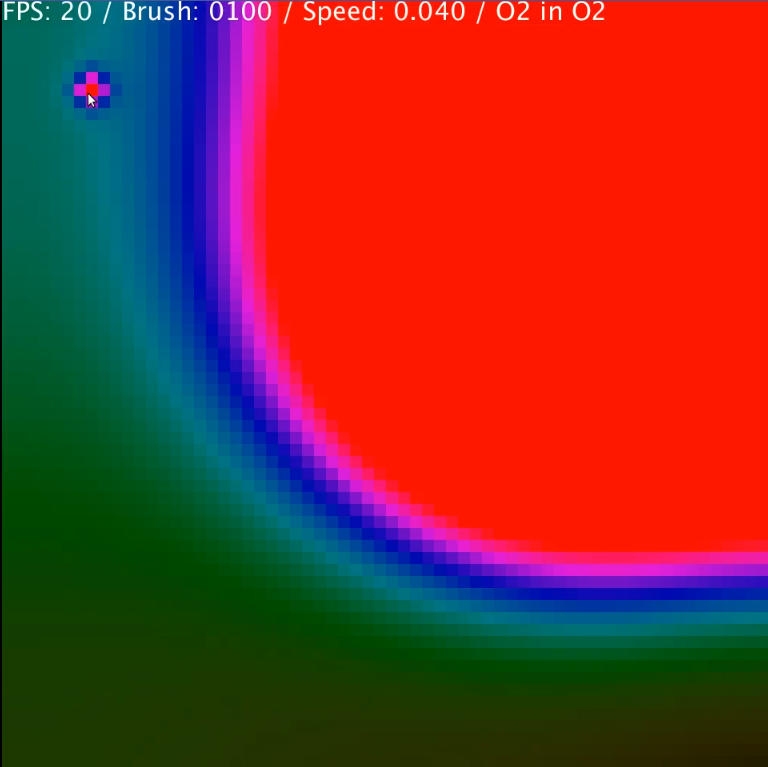
\includegraphics[scale=0.5]{pics/8.png}
\end{figure}

\pagebreak
The user can press N to clear the canvas and use the same fluid configuration and also add some fluid to the cleared canvas.

\begin{figure}[H]
	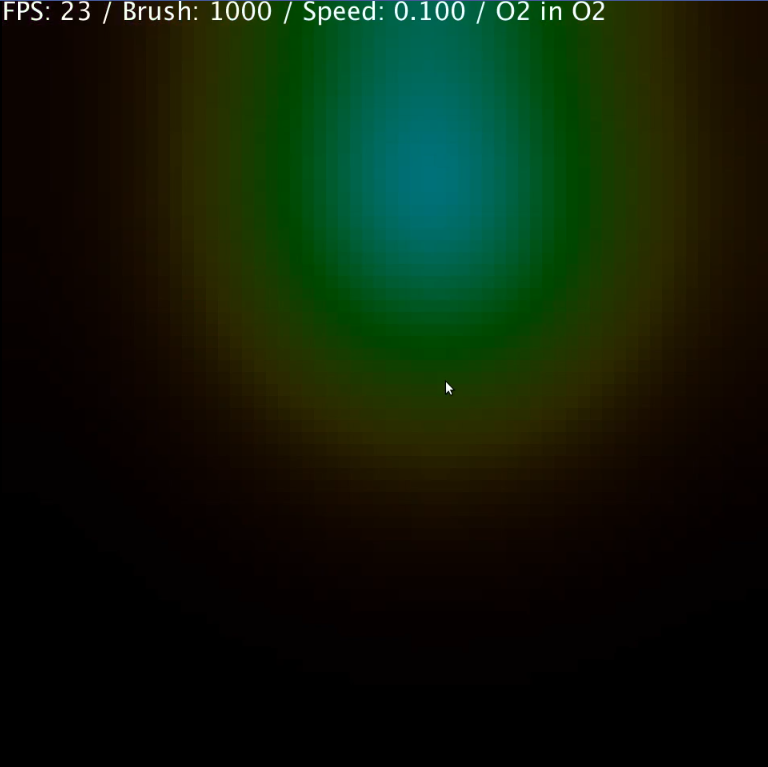
\includegraphics[scale=0.5]{pics/9.png}
\end{figure}

\pagebreak
Making the \verb|dt| very small with a will cause the diffusion and such be very slow. \verb|dt| can go down to 0.002 in increments of 0.002. Pressing a will increase \verb|dt| up to 0.1.

\begin{figure}[H]
	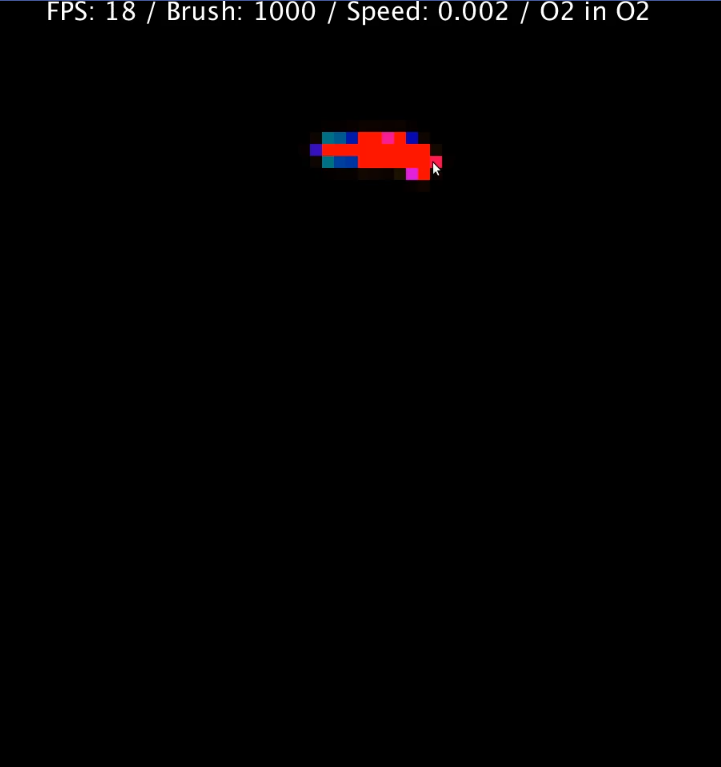
\includegraphics[scale=0.5]{pics/10.png}
\end{figure}

\pagebreak
Pressing F cycles through the different fluid configurations and clears the canvas.

\begin{figure}[H]
	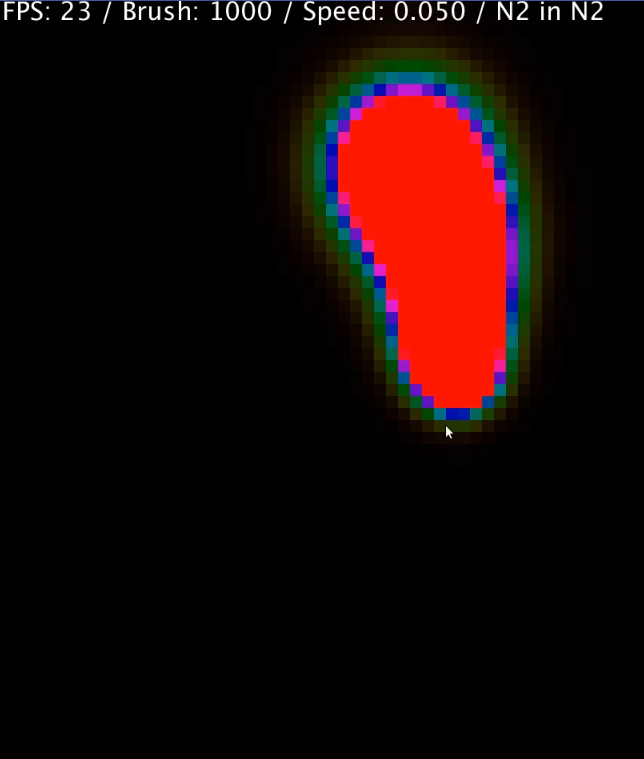
\includegraphics[scale=0.5]{pics/11.png}
\end{figure}

\pagebreak
The user can press c to toggle colour-coded mode. In the case that it is off, the pixels with density are displayed by shades of red.

\begin{figure}[H]
	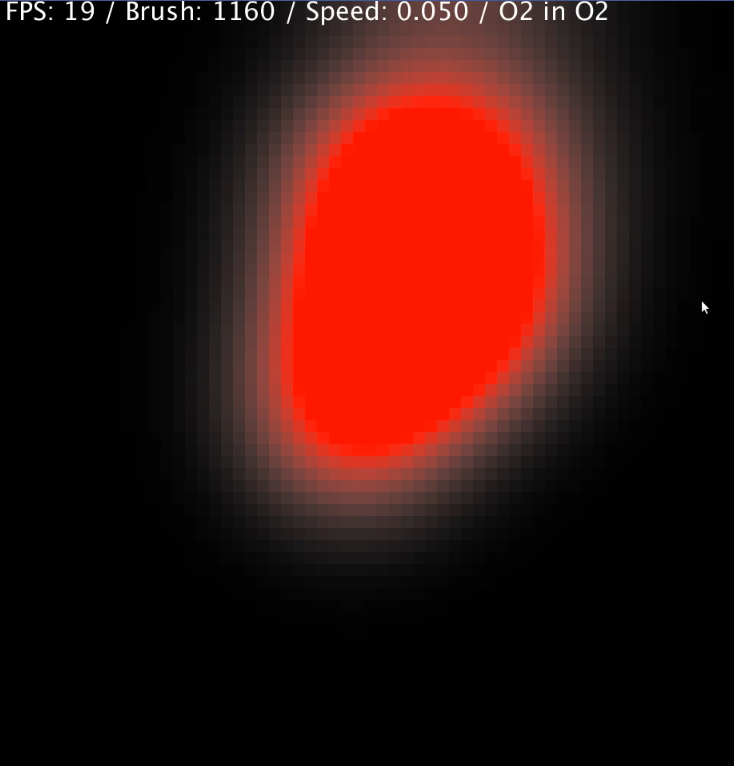
\includegraphics[scale=0.5]{pics/12.png}
\end{figure}

\pagebreak
Pressing d will toggle dark mode, changing the colour of the background and the colour of the UI.

\begin{figure}[H]
	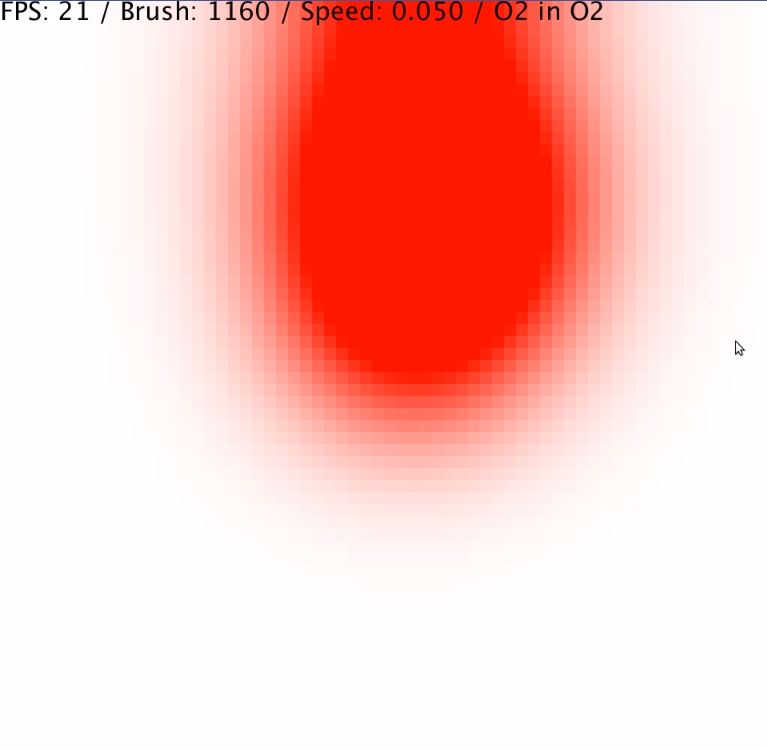
\includegraphics[scale=0.5]{pics/13.png}
\end{figure}

\pagebreak
And of course, you can use colour-coded mode while not being in dark mode.

\begin{figure}[H]
	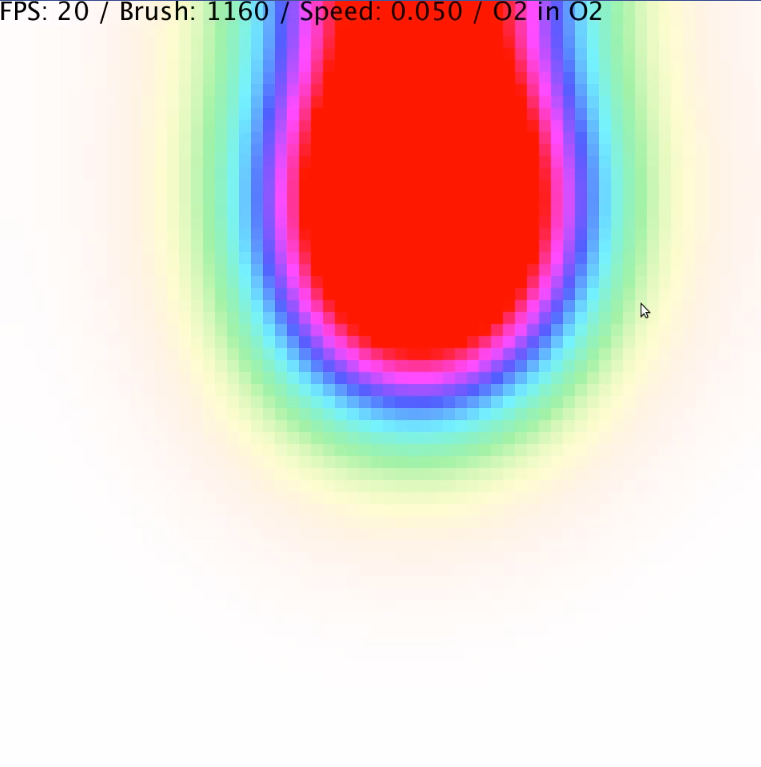
\includegraphics[scale=0.5]{pics/14.png}
\end{figure}

\chapter{System Testing}
Due to the nature of my program, there isn't a whole lot of testing required to make sure it is operational. The most important and error-prone part of the code is the solver, which is widely used and known to be correct. However, a few problems are outlined in the following sections. 

\section{Fixing array out of bounds when mouse is outside window}
This was the most major problem. As explained in the Code chapter, I added the \verb|ConstrainMouse| function to make sure that the solver receives non-erroneous values for the location of the density to be added. In order to be efficient I didn't write ad hoc checks for \verb|mouseX| and \verb|mouseY| - the variables containing the x and y coordinates of the mouse, correspondingly - instead i use a general value \verb|maxV| to take the value for both \verb|mouseX| and \verb|mouseY|. A selection is made to check if \verb|maxV| is excessive or negative and 0, because the boundary cells can't have a density:\\
\begin{lstlisting}
	int ConstrainMouse(int maxV, int val){
		if(val >= maxV){
			return maxV - 1;
		}
		if(val<=0){
			return 1; 
		}
		return val;
	}
\end{lstlisting}

\section{Diagnosing performance Issues regarding addition/subtraction of density}
I tried to write a custom function that detects if the mouse is pressed and call it while the simulation is running. However I discovered that using the built-in function \verb|mouseDragged()| offered by the processing.js default library, the FPS significantly increased. This is due to the fact that the built-in function only is called when, in this case, the mouse is dragged, where the user-defined function would be called every iteration of the loop, most of the times being unnecessary. A limitation of this is that the mouse has to be dragged \emph{and} clicked to add density.\\

\section{Ensuring Brush Size and Simulation Time Step are within range}
\verb|brush_size| is altered in the subroutine \verb|mouseWheel|, where there is a selection if its value exceeds \verb|max_brush_size| or is less than \verb|min_brush_size|, \verb|brush_size| is reset to the corresponding acceptable extreme - \verb|max_brush_size| or \verb|min_brush_size|. The handling of proper value of \verb|dt| is done in the subroutine \verb|SetSimulationSpeed|. The entire code of \verb|SetSimulationSpeed| is:
\begin{lstlisting}
	void SetSimulationSpeed(boolean increase){
		if(increase){
			dt+=0.002;
			if(dt>max_dt){dt=max_dt;}
		}
		else{
			dt-=0.002;
			if(dt<min_dt){dt=min_dt;}
		}
		GetFluid(choice);
	}
	
\end{lstlisting}
The value of \verb|dt| is increased/decreased unless it exceeds/is less than the valid extremes - \verb|min_dt| and \verb|max_dt|.\\


\section{Colour-coding}
Having only been familiar with RGB, I tried to use it to mimic an effect of colour-coding, which in my opinion makes the visualization more enjoyable. However, the colours were extreme and not to my liking. In retrospect, I realize I could've scaled down the values of each cell and then displayed them. However I found that if I instead used HSB, an alternative colour-coding convention, I could've given the user the ability to disable colour-coding. The code for the rendering of the density field is:
\begin{lstlisting}
	void RenderD(boolean dark, boolean code){
		noStroke();
		colorMode(HSB,100);
		
		for(int i=0;i<N;i++){
			for(int j=0;j<N;j++){
				int x = i * SCALE;
				int y = j * SCALE;
				
				float dr = this.dens[IX(i,j)];
				if(dark == true && code == true){fill(dr,255,dr);}
				else if (dark == false && code == false){fill(255,dr,255);}
				else if (dark == true && code == false){fill(0,dr,dr);}
				else if (dark == false && code == true){fill(dr,dr,255);}
				
				square(x,y,SCALE);
			}
		}
		
		
	}
\end{lstlisting}
\verb|colorMode(HSB,100);| means that that compiler will use HSB colour-coding with a maximum value of 100, meaning that cells containing a value greater than 100 will not be differently displayed than those with exactly 100. Having experimented with \verb|fill(value1,value2,value3);| which dictates the colour used for the pixel displayed (shown as a square), I found the above ways of colouring the square in all 4 possibilities (true/false dark, true/false code).\\



\section{UI}
I previously had a problem with the brush size not taking a constant space in letters, because "1000" has more characters than "999", so I simply add a "0" at the start of the brush size display if it is less than 1000. This amendment is found in \verb|RenderUI|:
\begin{lstlisting}
	void RenderUI(){
		textSize(32);
		colorMode(RGB);
		textMode(MODEL);
		if(dark){fill(255,255,255);}
		else{fill(0,0,0);}
		String message;
		if(brush_size<1000){message = "FPS: " + str(round(frameRate)) + " / Brush: 0" + str(brush_size) + " / Speed: " + String.format("%.3f", dt) + " / " + FluidName;}
			else{message = "FPS: " + str(round(frameRate)) + " / Brush: " + str(brush_size) + " / Speed: " + String.format("%.3f", dt) + " / " + FluidName;}
				text(message,0,25);
			}
\end{lstlisting}
Additionally, I had to inverse the colours of the background and UI text every time the value of \verb|dark| was changed, meaning when Dark Mode is cycled between on and off.



\chapter{Evaluation}

\section{Use}
The real-time fluid dynamics solver has an unlimited number of uses: in the development of video games the simulation of particles and fluids is key to the gaming experience, some crucial applications such as simulating the flow of air around a building to see if it is structurally sound, check airoplanes are stable at high speeds. I could go on but the applications are endless. The reader can think of my project as an application of the solver. It doesn't add much functionality to the original program, but it is a preliminary attempt at visualizing fluid flow in another fluid, which we have said is very useful. There already exist programs that trivialize the extent of my program, yet they couldn't have been developed so much without being what my project is, a preliminary visualization tool, at some point. Apart from that, having conversed with my physics teacher, this program and possibly a development of it can be used to convey laws of fluid dynamics to students in high school, such as Diffusion, Stoke's Law and Pascal's Principle, all of which fall under Chemistry and Physics A-Level (and even IGCSE) syllabus. I would imagine an advanced version of this can model the flow of blood through arteries and veins in Biology. All are exciting applications of my project and easily implemented, as the solver will not be changed. I myself find that the visualization of concepts that is physically modifiable is a very good way to learn. 



\section{Why I chose this Project Idea}
I am very interested in Physics and I plan on possibly following a career in computational physics. I always wanted to make this project Physics-related and I was enchanted by the endless uses of fluid dynamics in our lives that I had to do something related to them. I have made physics simulations and games for a long time, which although are trivial in their conception and code, meant a great deal to me. I am happy with this project, because I've always wanted to do it but could not find the diligence.


\section{Prospects for the Future}
The natural extension of the program is to convert it into a 3D simulation. The paper by Jos Stam that I based this project on makes clear that whoever understands the code can extend it into three dimensions. A more useful modification would be, in my opinion, to add obstacles in the simulation window that similarly to the boundary cells, can't exchange values of velocity and density, mimicking collision of the fluid. These obstacles could represent arteries, a building and everything that isn't a fluid, specifically a rigid solid (one that can't be bent). I could try to write the program in the programming language it's meant to be written in, C++. This would make the simulation much faster because C++ is a lower level language than Java and Python, hence being more efficient, but unnecessarily difficult for the purposes of this project. Believe me, I tried writing it in C++ and I immediately regretted it.



\chapter{Appendices}

\section{Appendix A: Java Code}
As previously mentioned, the code is Java-based and uses a JSON file for unique fluid configurations possible to simulate with the solver. Processing.js allowed me to export my code for Windows 32/64 bit and (my os) Linux 32/64 bit. The Java code for Linux in its entirety, barely being 350 lines:
\begin{lstlisting}
	import processing.core.*; 
	import processing.data.*; 
	import processing.event.*; 
	import processing.opengl.*; 
	
	import static javax.swing.JOptionPane.*; 
	
	import java.util.HashMap; 
	import java.util.ArrayList; 
	import java.io.File; 
	import java.io.BufferedReader; 
	import java.io.PrintWriter; 
	import java.io.InputStream; 
	import java.io.OutputStream; 
	import java.io.IOException; 
	
	public class sketch_201122a extends PApplet {
		
		
		
		Fluid fluid;
		JSONArray fluids;
		
		int choice = 0;
		String FluidName;
		Float FluidDiffusion, FluidViscosity;
		int brush_size = 1000;
		final int FrameRateCap=120;
		
		final int max_brush_size = 4000;
		final int min_brush_size = 100;
		boolean dark = true;
		boolean colorcode = true;
		
		int DSCALE = 100;
		
		
		
		public void settings(){
			size(N*SCALE,N*SCALE);
		}
		
		
		public void setup(){
			frameRate(FrameRateCap);
			InitUI();
			
			fluids = loadJSONArray("data/fluids.json");
			GetFluid(choice);
		}
		
		
		public void RenderUI(){
			textSize(32);
			colorMode(RGB);
			textMode(MODEL);
			if(dark){fill(255,255,255);}
			else{fill(0,0,0);}
			String message;
			if(brush_size<1000){message = "FPS: " + str(round(frameRate)) + " / Brush: 0" + str(brush_size) + " / Speed: " + String.format("%.3f", dt) + " / " + FluidName;}
				else{message = "FPS: " + str(round(frameRate)) + " / Brush: " + str(brush_size) + " / Speed: " + String.format("%.3f", dt) + " / " + FluidName;}
					text(message,0,25);
				}
				
				public void InitUI(){  
					String message = "The key bindings for the simulation are as follows:\nd : Toggle Dark Mode";
					message += "\nc : Toggle Color Coding\nn : Clear\nf : Cycle Through Fluids";
					message += "\nDrag Left Click : Add Fluid\nDrag Right Click : Remove Fluid\nScroll : Change Brush Size";
					message += "\ns : Lower Simulation Speed\na : Increase Simulation Speed";
					message += "\n\nThe legend of the UI is:\nFPS (" + str(FrameRateCap) + " max)  /  Brush Size /  Speed of Simulation  /  Fluid Configuration";
					
					showMessageDialog(null, message, "UI Help", INFORMATION_MESSAGE);
					
					
				}
				
				
				public int ConstrainMouse(int maxV, int val){
					if(val >= maxV){
						return maxV - 1;
					}
					if(val<=0){
						return 1; 
					}
					return val;
				}
				
				public void GetFluid(int newchoice){
					choice = newchoice%fluids.size();
					JSONObject fluids_choice = fluids.getJSONObject(choice);
					
					FluidName = fluids_choice.getString("configuration");
					FluidDiffusion = fluids_choice.getFloat("diffusion");
					FluidViscosity = fluids_choice.getFloat("viscosity");
					
					fluid = new Fluid(FluidDiffusion*DSCALE, FluidViscosity*DSCALE, dt);
				}
				
				
				public void SetSimulationSpeed(boolean increase){
					if(increase){
						dt+=0.002f;
						if(dt>max_dt){dt=max_dt;}
					}
					else{
						dt-=0.002f;
						if(dt<min_dt){dt=min_dt;}
					}
					GetFluid(choice);
				}
				
				public void mouseDragged(){
					
					float amountX = mouseX - pmouseX;
					float amountY = mouseY - pmouseY;
					
					int maxX = PApplet.parseInt(width/SCALE) - 1;
					int maxY = PApplet.parseInt(height/SCALE) - 1;
					
					if (mousePressed && (mouseButton == LEFT)){
						fluid.AddDensity(ConstrainMouse(maxX,mouseX/SCALE) , ConstrainMouse(maxY, mouseY/SCALE) , brush_size);
						fluid.AddVelocity(ConstrainMouse(maxX,mouseX/SCALE) , ConstrainMouse(maxY, mouseY/SCALE) , amountX*10, amountY*10);
					}
					if(mousePressed && (mouseButton == RIGHT)){
						fluid.AddDensity(ConstrainMouse(maxX,mouseX/SCALE) , ConstrainMouse(maxY, mouseY/SCALE), -brush_size);
					}
					
				}
				
				
				public void keyPressed(){
					if(key=='d'){dark = !dark;}
					if(key=='c'){colorcode = !colorcode;}
					if(key=='n'){GetFluid(choice);}
					if(key=='f'){GetFluid(choice+1);}
					if(key=='a'){SetSimulationSpeed(true);}
					if(key=='s'){SetSimulationSpeed(false);}
				}
				
				public void mouseWheel(MouseEvent event){
					float e = -1*event.getCount();
					brush_size += e*20;
					if(brush_size <= min_brush_size){brush_size=min_brush_size;}
					if(brush_size>=max_brush_size){brush_size=max_brush_size;}
				}
				
				public void draw(){
					background(0);
					
					fluid.step(dt);
					fluid.RenderD(dark,colorcode);
					
					RenderUI();
					
				}
				final int N=64;
				final int GRIDSIZE = (N+2)*(N+2);
				final int SCALE = 15;
				
				float dt = 0.04f;
				final float max_dt = 0.1f;
				final float min_dt = 0.002f;
				
				public int IX(int i, int j){
					return i + (N+2)*j; 
				}
				
				class Fluid{
					
					float dt;
					float diff;
					float visc;
					int size;
					
					float[] u;
					float[] v;
					float[] u_prev;
					float[] v_prev;
					
					float[] dens;
					float[] dens_prev;
					
					Fluid(float diffusion, float viscosity, float dtime){
						this.diff = diffusion;
						this.visc = viscosity;
						this.dt = dtime;
						
						this.dens_prev = new float[GRIDSIZE];
						this.dens = new float[GRIDSIZE];
						
						this.u = new float[GRIDSIZE];
						this.u_prev = new float[GRIDSIZE];
						this.v = new float[GRIDSIZE];
						this.v_prev = new float[GRIDSIZE];
					}
					
					public void step(float dtime){
						VelStep(u,v,u_prev,v_prev,visc,dtime);
						DensStep(dens,dens_prev,u_prev,v_prev,diff);
					}
					
					public void SetBnd(int b, float[] x){
						
						for (int i=1 ; i<=N ; i++ ) {
							x[IX(0 ,i)] = (b==1) ? -x[IX(1,i)] : x[IX(1,i)];
							x[IX(N+1,i)] = (b==1) ? -x[IX(N,i)] : x[IX(N,i)];
							x[IX(i,0 )] = (b==2) ? -x[IX(i,1)] : x[IX(i,1)];
							x[IX(i,N+1)] = (b==2) ? -x[IX(i,N)] : x[IX(i,N)];
						}
						x[IX(0 ,0 )] = 0.5f*(x[IX(1,0 )]+x[IX(0 ,1)]);
						x[IX(0 ,N+1)] = 0.5f*(x[IX(1,N+1)]+x[IX(0 ,N )]);
						x[IX(N+1,0 )] = 0.5f*(x[IX(N,0 )]+x[IX(N+1,1)]);
						x[IX(N+1,N+1)] = 0.5f*(x[IX(N,N+1)]+x[IX(N+1,N )]);
					}
					
					public void Advect(int b, float[] d, float[] d0, float[] u, float[] v){
						
						int i, j, i0, j0, i1, j1;
						float x, y, s0, t0, s1, t1, dt0;
						
						dt0 = dt*N;
						
						for(i=1;i<=N;i++){
							for(j=1;j<=N;j++){
								x = i-dt0*u[IX(i,j)]; y = j-dt0*v[IX(i,j)];
								if (x<0.5f) x=0.5f; if (x>N+0.5f) x=N+ 0.5f; i0=PApplet.parseInt(x); i1=i0+1;
								if (y<0.5f) y=0.5f; if (y>N+0.5f) y=N+ 0.5f; j0=PApplet.parseInt(y); j1=j0+1;
								s1 = x-i0; s0 = 1-s1; t1 = y-j0; t0 = 1-t1;
								d[IX(i,j)] = s0*(t0*d0[IX(i0,j0)]+t1*d0[IX(i0,j1)])+ s1*(t0*Snippetsd0[IX(i1,j0)]+t1*d0[IX(i1,j1)]);
								
								
							}
						}
						SetBnd(b,d);
						
					}
					
					public void Diffuse(int b, float[] x, float[] x0, float diff){
						
						float a = dt*diff*N*N;
						
						for(int k=0;k<20;k++){
							for(int i=1;i<=N;i++){
								for(int j=1;j<=N;j++){
									x[IX(i,j)] = (x0[IX(i,j)] + a*(x[IX(i-1,j)] + x[IX(i+1,j)] + x[IX(i,j-1)] + x[IX(i,j+1)]))/(1+4*a);
								}
							}
							SetBnd(b,x);
						}
						
					}
					
					
					public void AddDensity(int x, int y, float amount){
						int index = IX(x,y);
						this.dens[index] += amount;
					}
					
					public void AddVelocity(int x, int y, float amountX, float amountY){
						int index = IX(x,y);
						this.v[index] += amountX;
						this.u[index] += amountY;
					}
					Snippets
					public void Project(float[] u, float[] v, float[] p, float[] div){
						
						int i,j,k;
						float h;
						
						h = 1.0f/N;
						for(i=1;i<=N;i++){
							for(j=1;j<=N;j++){
								div[IX(i,j)] = -0.5f*h*(u[IX(i+1,j)]-u[IX(i-1,j)]+ v[IX(i,j+1)]-v[IX(i,j-1)]);
								p[IX(i,j)] = 0;
							}
						}
						SetBnd(0,div); SetBnd(0,p);
						
						for ( k=0 ; k<20 ; k++ ) {
							for ( i=1 ; i<=N ; i++ ) {
								for ( j=1 ; j<=N ; j++ ) {
									p[IX(i,j)] = (div[IX(i,j)]+p[IX(i-1,j)]+p[IX(i+1,j)]+ p[IX(i,j-1)]+p[IX(i,j+1)])/4;
								}
							}
							SetBnd(0, p);
						}
						
						for ( i=1 ; i<=N ; i++ ) {
							for ( j=1 ; j<=N ; j++ ) {
								u[IX(i,j)] -= 0.5f*(p[IX(i+1,j)]-p[IX(i-1,j)])/h;
								v[IX(i,j)] -= 0.5f*(p[IX(i,j+1)]-p[IX(i,j-1)])/h;
							}
						}
						SetBnd(1, u); SetBnd(2, v);
						
					}
					public void DensStep (float[] x, float[] x0, float[] u, float[] v, float diff ){
						Diffuse ( 0, x0, x, diff);
						Advect ( 0, x, x0, u, v);
					}
					
					public void VelStep(float[] u, float[] v, float[] u0, float[] v0, float visc, float dt){
						float[] tmp;
						
						
						tmp = u0; u0 = u; u=tmp;
						Diffuse(1,u,u0,visc);
						
						tmp = v0; v0 = v; v=tmp;
						Diffuse(2,v,v0,visc);
						
						Project(u,v,u0,v0);
						tmp = u0; u0 = u; u=tmp;
						tmp = v0; v0 = v; v=tmp;
						
						Advect(1,u,u0,u0,v0); Advect(2,v,v0,u0,v0);
						
						Project(u,v,u0,v0);
						
					}
					
					public void RenderD(boolean dark, boolean code){
						noStroke();
						colorMode(HSB,100);
						
						for(int i=0;i<N;i++){
							for(int j=0;j<N;j++){
								int x = i * SCALE;
								int y = j * SCALE;
								
								float dr = this.dens[IX(i,j)];
								if(dark == true && code == true){fill(dr,255,dr);}
								else if (dark == false && code == false){fill(255,dr,255);}
								else if (dark == true && code == false){fill(0,dr,dr);}
								else if (dark == false && code == true){fill(dr,dr,255);}
								
								square(x,y,SCALE);
							}
						}
						
						
					}
					
				}
				static public void main(String[] passedArgs) {
					String[] appletArgs = new String[] { "sketch_201122a" };
					if (passedArgs != null) {
						PApplet.main(concat(appletArgs, passedArgs));
					} else {
						PApplet.main(appletArgs);
					}
				}
			}
\end{lstlisting}

\pagebreak

\section{Appendix B: JSON File}
	
The JSON file I created containing realistic configurations of fluids in other fluids is found in data/fluids.json:
\begin{verbatim}
	[
	{"configuration":"O2 in O2", "diffusion":0.0000198, "viscosity":0.0000176},
	{"configuration":"N2 in N2", "diffusion":0.0000189, "viscosity":0.0000204},
	{"configuration":"C02 in C02", "diffusion":0.0000104, "viscosity":0.0000147},
	{"configuration":"O2 in Air", "diffusion":0.0000178, "viscosity":0.0000182},
	{"configuration":"N2 in Air", "diffusion":0.0000138, "viscosity":0.0000182},
	{"configuration":"C02 in Air", "diffusion":0.0000236, "viscosity":0.0000182}    
	]
\end{verbatim}


\section{Appendix C: GitHub}
In order to avoid confusion, I attach a link to a GitHub repository containing all files produced: \href{https://github.com/AnastasiosZ/A2-Project-FluidSim}{https://github.com/AnastasiosZ/A2-Project-FluidSim}


\begin{thebibliography}{9}
	\bibitem{josrtfdg} Real-Time Fluid Dynamics for Games, Jos Stam, GDC 2003 Conference proceedings, 2003.
	\bibitem{fsfd} Fluid Simulation for Dummies, Michael Ash, blog post 2006 (\href{https://mikeash.com/pyblog/fluid-simulation-for-dummies.html}{https://mikeash.com/pyblog/fluid-simulation-for-dummies.html}).
	\bibitem{mikeaskmthesis} Simulation and Visualization of a 3D Fluid, Michael Ash, Master's Thesis 2005.
	\bibitem{codingtrain132} CC 132 Fluid Simulation, (\href{https://github.com/CodingTrain/website/tree/main/CodingChallenges/CC_132_FluidSimulation/Processing/CC_132_FluidSimulation}{https://github.com/CodingTrain/website/tree/\\main/CodingChallenges/CC\_132\_FluidSimulation/Processing/CC\_132\_FluidSimulation})
\end{thebibliography}

\end{document}